%
% حق نشر 1390-1402 دانش پژوهان ققنوس
% حقوق این اثر محفوظ است.
% 
% استفاده مجدد از متن و یا نتایج این اثر در هر شکل غیر قانونی است مگر اینکه متن حق
% نشر بالا در ابتدای تمامی مستندهای و یا برنامه‌های به دست آمده از این اثر
% بازنویسی شود. این کار باید برای تمامی مستندها، متنهای تبلیغاتی برنامه‌های
% کاربردی و سایر مواردی که از این اثر به دست می‌آید مندرج شده و در قسمت تقدیر از
% صاحب این اثر نام برده شود.
% 
% نام گروه دانش پژوهان ققنوس ممکن است در محصولات دست آمده شده از این اثر درج
% نشود که در این حالت با مطالبی که در بالا اورده شده در تضاد نیست. برای اطلاع
% بیشتر در مورد حق نشر آدرس زیر مراجعه کنید:
% 
% http://dpq.co.ir/licence
%
%استفاده از {\lr{Doxygen}} به صورت گرافیکی (با استفاده از {\lr{Doxywizard}})
\section{گرافیکی (با استفاده از \lr{Doxywizard})}

\lr{Doxywizard} 
یک برنامه گرافیکی برای پیکربندی و اجرای \lr{doxygen} است. با اجرای این برنامه یک
پنجره اصلی (که بسته به سیستم عاملی که دارید ظاهر آن متفاوت است) نمایش داده
می‌شود(برای نمونه تصویر \ref{پنجره_داکسی_ویزارد} را ببینید).
با استفاده از امکانات گرافیکی موجود در این برنامه می‌توان \lr{doxygen} را
پیکربندی و اجرا کرد. به طور کلی با استفاده از \lr{doxywizard} می توان کارهای زیر
را انجام داد:

\begin{itemize}
 \item
پیکربندی \lr{doxygen} و ذخیره آن به صورت یک پرونده متنی برای استفاده‌های بعدی.
\item
باز کردن و ویرایش یک پرونده پیکربندی که از قبل تهیه شده.
\item
اجرای \lr{doxygen} برای تولید مستندات بر اساس پیکربندی تعیین شده.
\end{itemize}

\begin{figure}
\centering
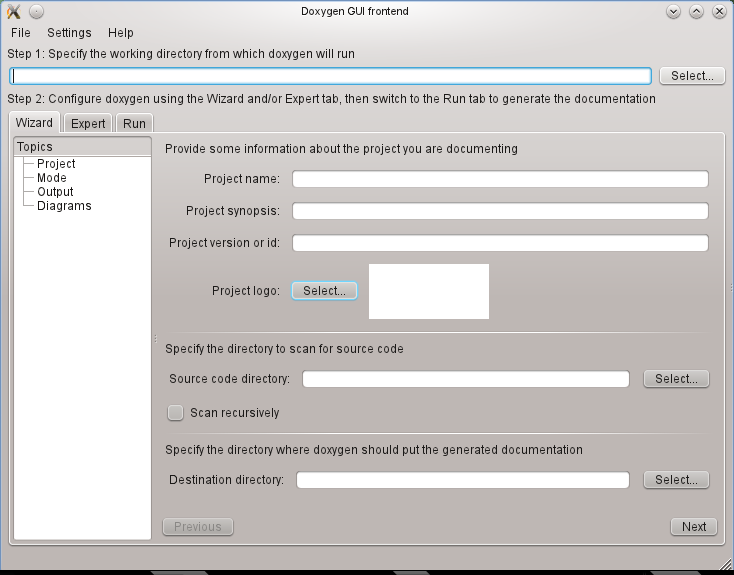
\includegraphics[width=0.75\textwidth]{image/doxywizard_linux}
\caption[نمونه‌ای از پنجره اصلی برنامه گرافیکی \lr{Doxywizard}.]
{
نمونه‌ای از پنجره اصلی برنامه گرافیکی \lr{Doxywizard}. با استفاده از امکانات گرافیکی موجود در این برنامه می‌توان پرونده‌های پیکربندی را تهیه و ویرایش کرد و برنامه \lr{Doxygen} را نیز به اجرا درآورد.
}
\label{پنجره_داکسی_ویزارد}
\end{figure}


همانطور که قبلاً هم گفته شد، برای تولید مستندات از کدهای منبع با استفاده از
\lr{dowygen} ابتدا باید یک پرونده پیکربندی تهیه کرد تا \lr{doxygen} بر اساس آن
اقدام به تولید مستندات کند. در ادامه توضیح داده می‌شود که چگونه می‌توان با
استفاده از امکانات گرافیکی موجود در \lr{doxywizard} یک پرونده پیکربندی تهیه کرد
و \lr{doxygen} را اجرا کرد.

\subsection{پیکربندی}

برای پیکربندی \lr{doxygen} از طریق \lr{doxywizard} سه روش وجود دارد که در ادامه
این روش‌ها را شرح می‌دهیم.

\paragraph{روش اول: استفاده از پرونده پیکربندی از قبل موجود.}
در صورتی که یک پرونده پیکربندی آماده دارید و اکنون می‌خواهید همان پیکربندی را به
کار ببرید و یا اینکه می‌خواهید آن را کمی ویرایش کنید و سپس از آن استفاده کنید،
می‌توانید از منوی \lr{File} گزینه \lr{Open} را انتخاب کنید (البته در برخی موارد
دکمه‌ای تحت عنوان \lr{Load} برای این کار است وجود دارد). با این کار
\lr{doxywizard} پرونده مربوطه را خوانده و تنظیمات درج شده در آن را در قسمت‌های
مختلف نمایش می‌دهد. در صورت نیاز می‌توانید هر قسمت را که می‌خواهید ویرایش کنید.

\paragraph{روش دوم: پیکربندی سریع.}
در صورتی که بخواهید فقط تنظیمات مهم را تعیین کنید و سایر جزئیات و تنظیمات را با
مقدار پیش‌فرض رها کنید تب \lr{Wizard} را انتخاب کنید. با انتخاب این تب در فهرست
سمت چپ چهار آیتم \lr{Project}، \lr{Mode}، \lr{Output} و \lr{Diagram} را مشاهده
خواهید کرد. این چهار آیتم در واقع چهار مرحله برای تنظیمات است. در هر مرحله
تنظیمات خاصی تعیین می‌شود. در زیر این مراحل شرح داده شده است:

\subparagraph{\lr{Project}}
در این قسمت تنظیمات عمومی مربوط به پروژه‌ای که مستندات آن تولید خواهد شد تعیین
می‌شود. این تنظیمات عبارتند از:
نام پروژه، خلاصه‌ای از پروژه، شماره نسخه پروژه، لوگوی پروژه و آدرس پوشه‌ای که
پرونده‌های منبع (کدها و توضیحات) پروژه در آن قرار دارد. علاوه بر آن‌ها گزینه‌ای
تحت عنوان \lr{Scan recursively} وجود دارد. این گزینه برای مواقعی است که درون
پوشه حاوی کدهای منبع، پوشه‌های دیگری نیز وجود داشته باشد که پرونده‌های درون این
پوشه‌ها هم باید در تولید مستند استفاده شوند (به عبارتی پروژه حاوی پوشه‌های تو در
تو باشد). آخرین آیتم این مرحله تعیین آدرس پوشه‌ای است که مستندات تولید شده توسط
\lr{doxygen} باید در آن قرار گیرند (یعنی آدرس پوشه نتایج).

در بالاترین قسمت پنجره \lr{doxywizard} محلی وجود دارد که در آن می‌توان پوشه‌ یا
آدرسی را که \lr{doxygen} باید در آن اجرا شود، تعیین کرد. اگر آدرس پوشه
پرونده‌های منبع یا پوشه نتایج زیر پوشه‌ای از آدرس داده شده باشند، می‌توان آدرس
آن‌ها را به صورت نسبی، نسبت به پوشه مذکور وارد کرد. در غیر این صورت باید حتما
آدرس‌ها به صورت مطلق داده شوند.

\subparagraph{\lr{Mode}}
در این قسمت نحوه استخراج مستندات از کدها منبع تعیین می‌شود. در بخش اول تعیین
می‌شود که آیا کلیه موجودیت‌ها (کلاس‌ها، متدها، توابع و \ldots) در مستند تولیدی
آورده شوند (\lr{All Entities}) یا اینکه فقط موجودیت‌هایی که مستند شده‌اند در
مستند ظاهر شوند (\lr{Docuented entities only}).

در صورتی که بخواهید ارجاعات یا پیوندهایی به اصل کدها در مستندات وجود داشته باشد
باید گزینه \lr{Include cross-referenced \ldots} تیک زده شود (این کار در واقع
معادل با مقداردهی تگ \lr{SOURCE\_BROWSING} با مقدار \lr{YES} در پرونده پیکربندی
است).

در بخش دوم این تب می‌توان زبان برنامه‌نویسی پروژه را تعیین کرد تا مستندات تولیدی
برای زبان مربوطه بهینه شود.

\subparagraph{\lr{Output}}
این قسمت تنظیمات مربوط به خروجی‌های \lr{doxygen} است. در این قسمت می‌توان تعیین
کرد که مستندات در چه قالبی تولید شوند. قالب‌های ممکن عبارتند از: \lr{HTML}،
\lr{\LaTeX}، \lr{Man page}، \lr{RTF} و \lr{XML}.
برای دو قالب \lr{HTML} و \lr{\LaTeX} تنظیمات بیشتری نیز وجود دارد.

در قسمت \lr{HTML} می‌توان تعیین کرد که مستندات تولید شده در قالب \lr{HTML} فقط
حاوی \lr{HTML} ساده باشد، حاوی بخش دسترسی سریع\footnote{\lr{Navigation panel}}
باشد یا اینکه در قالب \lr{.chm} باشد. همچنین می‌توان تعیین کرد که قسمت جستجو در
صفحات \lr{html} وجود داشته باشد یا نه. برای این کار باید گزینه \lr{With search
function} را علامت‌دار یا بدون علامت کرد.

در تنظیمات مربوط به قالب \lr{HTML} دکمه‌ای تحت عنوان \lr{Change color \ldots}
وجود دارد که با استفاده از آن می‌توان رنگ عمومی صفحات \lr{HTML} را تعیین کرد. با
فشردن این دکمه پنجره‌ای نمایش داده می‌شود که در سمت راست آن سه نوار رنگی قرار
دارد. با تغییر فلش مربوط به این نوارهای رنگی می‌توانید رنگ مورد نظر خود را تعیین
کنید.


در قسمت \lr{LaTeX} می‌توان تعیین کرد که مستندات در قالب \lr{\LaTeX} به عنوان یک
قالب میانی برای تولید \lr{PDF} است یا \lr{PostScript}.

به این نکته توجه داشته باشید که در هر صورت \lr{Doxygen} پرونده‌های مربوط به
کدهای منبع را تغییر نمی‌دهد و فقط آن‌ها را می‌خواند.

\subparagraph{\lr{Diagram}}
\lr{Doxygen} 
می‌تواند دیاگرام‌هایی را در مستندات تولید کند. در این قسمت تعیین می‌شود که چه
دیاگرام‌هایی و چگونه تولید شوند.
بیشتر دیاگرام‌ها به ابزار \lr{dot} از بسته \lr{GraphViz}\footnote{ برای کسب
اطلاعات بیشتر درباره این بسته نرم‌افزاری و دریافت آن می‌توانید به آدرس
\lr{http://www.graphviz.org} مراجعه نمایید.} نیاز دارند. در حالت کلی سه گزینه
برای انتخاب وجود دارد: مستندات بدون دیاگرام تولید شوند، از تولید کننده داخلی
برای تولید کلاس دیاگرام استفاده شود، یا اینکه از ابزار \lr{dot} از بسته
\lr{GraphViz} برای تولید دیاگرام استفاده شود.

\paragraph{روش سوم: پیکربندی با جزئیات کامل.}
برای دسترسی به کلیه تنظیمات ممکن در پرونده پیکربندی و ویرایش تنظیمات مورد نظر
می‌توان از تب \lr{Expert} استفاده کرد. در این قسمت تمام تنظیماتی که در یک پرونده
پیکربندی \lr{doxygen} وجود دارد قابل مشاهده است. برای نظم بیشتر و دسترسی راحت‌تر
این تنظیمات در در ۱۶ گروه دسته‌بندی شده‌اند. نام گروه‌ها در فهرست سمت چپ در تب
\lr{Expert} مشاهده می‌شود.
البته به این نکته توجه داشته باشید که می‌توانید تنظیمات مورد نظر خود را از
قسمت‌های مختلف (هم از قسمت \lr{Wizard} و هم از قسمت \lr{Expert}) تعیین کنید.

اگر محتویات یک پرونده پیکربندی را مشاهده کنید می‌بینید که تنظیمات مختلف به نوعی
دسته‌بندی شده‌اند. گروه‌های مختلفی که در فهرست سمت چپ از تب \lr{Expert} مشاهده
می‌کنید در واقع همان دسته‌بندی را نشان می‌دهند که در اینجا نمایی گرافیکی دارد.
در هر گروه از تب \lr{Expert}، برای هر مورد قابل تنظیم (به عبارتی برای هر تگ) در
پرونده پیکربندی یک عنصر گرافیکی تهیه شده است. عنصر گرافیکی مربوط به هر تگ، به
نوع آن تگ و  مقدار یا مقادیری که می‌تواند بگیرد بستگی دارد.

% مطالب مربوط به صفحه ۸۴ از مستند کاربری داکسی ژن
\begin{itemize}
 \item 
برای تنظیماتی که از نوع بولی (تنظیماتی که در پرونده پیکربندی با مقادیر \lr{YES} یا \lr{NO} مقداردهی می‌شوند دکمه‌ای 
برای علامت زدن (یا \lr{check-box}) وجود دارد.
\item
برای تنظیماتی که می‌توانند مقادیر خاص و معین بگیرند (مثل تگ \lr{OUTPUT\_LANGUAGE} که زبان مستندات تولید شده را 
تعیین می‌کند) یک فهرست انتخاب (یا \lr{combo box} در نظر گرفته شده است.
\item
برای تنظیماتی که مقادیر عددی از بازه‌ای خاص را می‌توانند بگیرند یک \lr{spinbox} در نظر گرفته شده است.
\item
برای تنظیماتی که می‌توانند یک رشته (یا یک جمله) را به عنوان مقدار دریافت کنند، یک جعبه ویرایش تک 
خطی (\lr{one line edit field}) در نظر گرفته شده است.
\item
برای تنظیماتی که می‌توانند چند رشته (یا چند کلمه) را به عنوان مقدار دریافت کنند (مثل تگ \lr{FILE\_PATTERNS}) یک 
جعبه ویرایش تک خطی به همراه سه دکمه '+'، '-' و '*' و یک فهرست در نظر گرفته شده است. با نوشتن یک رشته در جعبه 
ویرایش و زدن دکمه '+' رشته مورد نظر به فهرست اضافه می‌شود. با انتخاب یک رشته از فهرست و زدن دکمه '-' آن رشته 
حذف می‌شود. با انتخاب یک رشته از فهرست و تغییر آن و سپس زدن دکمه '*' تغییرات داده شده در رشته انتخاب شده در فهرست 
اعمال می‌شود (به عبارتی رشته جدید با رشته قبلی جایگزین می‌شود).
\item
برای تنظیماتی که یک پرونده یا یک پوشه را به عنوان مقدار دریافت می‌کنند دکمه‌ای وجود دارد که با فشردن آن، پنجره‌ای 
برای انتخاب پرونده یا پوشه ظاهر می‌شود.
\end{itemize}

برای مشاهده توضیحات مربوط به هر آیتم یا معنی آن، کافی است اشاره‌گر ماوس را روی
آیتم مورد نظر ببرید. در این حالت در پنجره‌ای که در قسمت پایین سمت چپ قرار دارد
توضیحاتی در مورد آیتم نمایش داده می‌شود (در برخی موارد در قسمت پایین سمت راست
دکمه‌ای تحت عنوان راهنما (\lr{Help}) قرار دارد که با زدن این دکمه و سپس کلیک روی
آیتم مورد نظر، توضیحات مربوط به آن آیتم به نمایش درمی‌آید).

\subsection{اجرای \lr{Doxygen}}

برای اجرای \lr{doxygen} از طریق \lr{doxywizard} باید تب \lr{Run} را انتخاب کنید.
در این تب می‌توانید تنظیماتی که تعیین کرده‌اید را ببینید. برای مشاهده دکمه
\lr{Show configuration} را بزنید. با این کار کلیه تنظیمات (هم آن‌هایی که ویرایش
کرده‌اید، هم آن‌ها که به صورت پیش‌فرض رها کرده‌اید) مشاهده می‌شود که از طریق
دکمه \lr{Save log} می‌توانید آن‌ها را در به صورت یک پرونده متنی ذخیره کنید تا در
صورت نیاز بعداً به صورت دستی و یا از طریق همین برنامه \lr{doxywizard} آن را باز
کرده و ویرایش کنید.

با زدن دکمه \lr{Run doxygen} یا \lr{Start} برنامه \lr{doxygen} با توجه به
تنظیماتی که تعیین کرده‌اید شروع به کار می‌کند و در حین تولید مستندات، گزارشی از
کارهایی که در حال انجام است نیز نمایش داده می‌شود. این گزارش‌ها را نیز می‌توان
از طریق همان دکمه \lr{Save log} به عنوان یک پرونده متنی ذخیره کرد. هنگام اجرای
\lr{doxygen} اگر از ادامه کار منصرف شدید می‌توانید با زدن همان دکمه قبلی از
ادامه کار \lr{doxygen} جلوگیری کنید.

پس از اتمام تولید مستندات توسط \lr{doxygen}، می‌توان از طریق دکمه \lr{Show HTML
output} به صفحه اول مستندات تولیدی در قالب \lr{HTML} رجوع کرد. البته در صورتی که
در پیکربندی اولیه، تولید مستندات در قالب \lr{HTML} را فعال نکرده باشید این دکمه
غیرفعال خواهد بود زیرا \lr{doxygen} مستندی در قالب \lr{HTML} تولید نکرده است.